\chapter{Research Methodology}
%\label{chapter:Research Methodology}
\emph{The research methodology describes a chronological order of methodologies used to execute research. Components are research philosophy and approach, research design, data collection and preparation, data-driven sparse-sensing techniques and QR-based algorithm, and a case study in which two study areas are discussed.}

\section{Research philosophy and approach}
Within this research study, a positivism research philosophy is adopted. Positivism can be illustrated as a scientific conception to which a phenomenon can be known through empirical data based on natural processes. The concept relies on quantitative measurements and methods to illustrate the hydrological phenomenon and predict it in this way. As stated by Kabo et al. (2022), a mathematical model of hydrological flow is based on a positivist paradigm through which the natural world can be explained. According to Jansen (2023), a research methodology with a positivist perspective can only acquire data through measurements and observations. Data used in this research study is acquired through manual and sensor measurements of monitoring wells inherited by the City of Rotterdam. Next to the research philosophy, the research approach that is planned to be adopted is a quantitative research method. This research method involves the collection and analysis of numerical data to test hypotheses, examine patterns, and establish relationships between variables. The objective is to quantify and generalize findings. A quantitative research method uses a deductive approach, meaning a clear theory or hypothesis has to be researched. Consequently, the theory or hypothesis is tested, using specific observations or data. The research approach uses a top-down approach, meaning the theory or hypothesis that is available is first assessed instead of assessing data or observations (Jansen, 2023). 
\newpage
\section{Research design }
\emph{Following with the research design. The research design of this study describes the overall plan and guides the research study based on the objective.} 
The research study has the purpose to generate a generic model in order to examine the degree of optimization of the GWMN of Rotterdam's municipal area. The approach employs a two-part research design: 
\textbf{\subsubsection{Descriptive Design}}
The initial phase aims to characterize the present state of the system, utilizing hydrogeological and geographical data of the research areas. The system description involves analyzing the distribution and coverage of monitoring wells in the municipality without manipulating variables. The descriptive design develops a detailed visualization of the existing GWMN, including parameters as distribution, coverage density, and groundwater level measurements.

\textbf{\subsubsection{Quasi-experimental Design}}
The second phase includes an approach that manipulates the GWMN by simulating data and adding, relocating and removing monitoring wells. These actions have the purpose to observe changes regarding network optimization. Initially, the research study includes 14 city districts and 4 industrial areas, however, a generic model is set-up. Therefore, only two specific research areas are included in the chapter "Results". The choice of the two specific research areas is based on factors as measurement type (data loggers or manual measurements), monitoring frequency, density of the coverage area, as well as factors as frequency of water-related issues in the study area. Data loggers ensure that inaccessible and vulnerable locations within the city districts can still be frequently monitored through this approach. Certain monitoring wells are on inaccessible locations within the municipal area, however, through the data loggers they can still be monitored. The second phase aims to analyze the impact of the changes regarding network optimization quantitatively over a longitudinal period.\\
\\

\section{Data collection and preparation}
Within this research study, the time period includes 01-01-2010 to present date (19-01-2024). From 2010 to 2014, groundwater data is collected by the municipality of Rotterdam. Field service employees of the field measurement service collected data through manual measurements. The measurements took place at the end of the month, trying to sample every four weeks and taking into account personal circumstances of the field employees. In the period of 2014 to 2018, the field measurements were carried out by an external contracting company. The transition to different field service employees in 2014 and 2018 possibly ensures that errors and differences can arise in the approach of collecting data. Since 2019, groundwater data is collected by the municipality of Rotterdam again. This also means that multiple monitoring wells were passed to data loggers instead of manual measurements. Because of this transition, inaccessible locations were still monitored and data is collected more frequently, per day instead of per month.

\subsection{QGIS and PROWAT}
The open-source Geographic Information System (qGIS) of the municipality of Rotterdam as well as the application Sensor Management allow the availability of monitoring data for all unique monitoring wells within the municipal area. In qGIS, study areas of preference can be selected and transferred to the PROWAT system. PROWAT allows the data to be converted to an Excel data file. After which data can be imported in the machine learning program Python. 

\subsection{Pastas Time Series Modeling}
The quasi-experimental research design starts with Pastas, a Python package made to analyze a sequence of data points that are collected over specific intervals of time (Artesia, n.d.). Data gaps are present in the dataset,  resulting in potential problems later on in the development of the model. At first, a basic model is generated to visualize a simple time series model to simulate groundwater levels.

\textbf{\subsubsection{Dependent Time Series}}

A time series of groundwater levels is imported through the Pandas package. The dependent time series data describes the observed time series monitored by the municipality of Rotterdam. The figure describes the groundwater level [m MSL] over a period of 22-09-2010 to 22-08-2023. Unique monitoring wells of the neighborhood of Rozenburg are visualized. It is the intention that seasonal fluctuations, high and low variabilities are easily visualized in the plot. 
\\
\textbf{\subsubsection{Independent Time Series}}

A next step of the Pastas time series modeling consists of importing the independent time series from an external dataset. In order to import the independent time series, two explanatory series are implemented. Precipitation and potential evaporation are the explanatory series. With use of precipitation and potential evaporation data, recharge to the groundwater can be calculated. The data of the precipitation and evaporation data is conducted by the Royal Netherlands Meteorological Institute at weather station 344 in Rotterdam (KNMI, 2024). The resulting figure describes the recharge level [m/day] over a time period of 22-09-2010 to 19-01-2024. 

\textbf{\subsubsection{Time Series Model}}

After the dependent time series (based on observed GWL data) and independent time series (based on precipitation and evaporation data) are developed and plotted, the actual time series model is created. The dependent and independent time series are imported to the actual time series model. The imported time series are approved for missing values or inconsistencies in data. The model is solved through assessing optimal model parameters. The solution of the calculation can be plotted in a time series plot. The plot describes the observed data as a scatter plot and the simulation data, according to the independent data in a line plot. The actual time series model includes "Stress Model 1".

The observed data translates the groundwater level [m MSL] over a time period of 22-09-2010 to 19-01-2024. Besides the time series plot of the calculation, it is possible to accommodate an overview of the model. In the overview plot, the previous figure is plotted as well as a subplot of the residuals and noise, recharge and stresses, model parameters, and confidence interval. 

\textbf{\subsubsection{Statistical Substantiation}}

Next to that, a summary of the developed statistical metrics are shown in a table overview. The performance of the models is visualized through a bar plot. Statistical metrics regarding the RMSE, R2, and EPV are shown. Nevertheless, based on the statistical data only it can not be proved that a model is performing "good" or "bad". Therefore, additional statistical tests are executed. The Welch's t-test compares two data groups, "datalogger" and "manual measurement", within the dataset. The t-test is carried out to criticize whether a dataset with a combination of measurement types: datalogger, manual or a combination of both of them is recommended to be used. Nonetheless, in the context of environmental sciences, looking beyond statistical significance is key. Other factors such as a reliability and data quality, confidence intervals, and the preference of stakeholders for example can shape the final decision regarding the choice of the data group. Overall, it is fundamental to consider a holistic approach that includes more factors bedsides statistical significance. Consequently, the decision is made to continue the research study with use of the data group "datalogger". The observed and simulated data of the measurement type "datalogger" are merged into a new data frame that is used in the next step "QR Factorization". 

\newpage
\section{QR Factorization}
A data-driven algorithm is designed to optimize groundwater monitoring networks by determining the optimal number and location of monitoring wells for temporal and spatial level reconstruction. The algorithm can be explained by the dependency of data in order to make a certain decision, prediction or optimization process. Existing data from the municipality is used to study patterns, trends, and relationships between parameters. The method was first obtained by Ohmer et al. (2022) at the KIT and applied the methodology to a study area in Germany. The approach is included in the optimization approach regarding the municipality of Rotterdam. The network reduction method is utilized on the GWMN, using one-dimensional hydrograph data. The main process of the algorithm is the use of QR factorization, a mathematical approach that breaks down matrix A into the product of two matrices: Q and R. Q is an orthogonal matrix that transforms the original dataset into a new dataset with independent columns. This is essential for evaluating the unique contribution of each monitoring well. On the other hand, R is a triangular matrix, where values below the diagonal are equal to zero. The triangular matrix serves to rank monitoring well based on their informational relevance. Figure 4.1, visualizes the decomposition of product A into matrices Q and R (Hinno, 2021).

\begin{figure}[htbp]
    \centering
    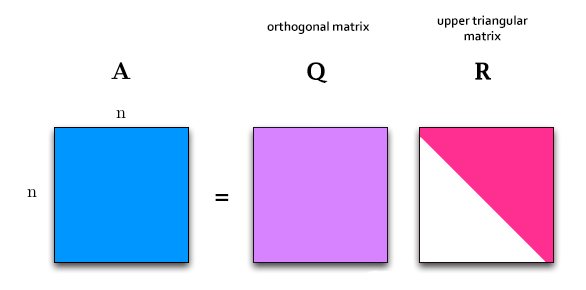
\includegraphics[width=0.40\linewidth]{figures/figures theory/qr rank.png}
    \caption{QR decomposition process from product A into matrices Q and R.}
\end{figure}
The optimization approach enables the network to be reduced along the Pareto front, balancing information loss against cost savings. To achieve the most accurate reconstruction with the least number of monitoring wells, the algorithm tests various reduction scenarios (25-50-75-90 percent) to identify the lowest reconstruction error. It can, however, be possible that the optimal reduction percentage differs between the study areas. A reduction percentage of at least 25 percent should be applied to describe the system dynamics in the study areas, while a reduction percentage exceeding 75 percent would influence the accuracy of the reduction results, states Ohmer et al. (2022). \\
\\
Appendix B describes a detail script regarding the QR factorization method. The Python package "PySensors" contains a data-driven algorithm for sparse sensor selection and signal reconstruction with dimensional reduction.





\newpage
\section{Data Analysis}
In terms of data analysis, the study is divided into two components:
\textbf{\subsubsection{Descriptive design}}
The purpose is to analyze the current conditions of the municipal area. This includes hydrogeological and geographical system descriptions of the municipal area as well as the study area. Based on the surface area of the chosen study areas, public spaces and the number of monitoring wells, the ratio of coverage can be calculated and analyzed.
\
\textbf{\subsubsection{Quasi-experimental design}}
The design objective is to construct a generic model to evaluate the level of optimization achieved. This includes an analysis of the distribution and effectiveness of monitoring wells within selected study locations. The analysis utilizes groundwater level data collected by data loggers and manual readings to enable time series analysis and modeling. A first step is choosing a precise data group within the dataset. The choice is substantiated by the application of a Welch's t-test. The t-test has a decision-making role in choosing the most reliable data collection method, necessary for the completeness of the QR factorization model. Once the data set is complete, the data is converted to the correct file shape where the data frames are centered on global and local scale. This means that the mean value as well as the minimum and maximum value of the groundwater level data is determined. The dataset is divided into training and test data, an 80 to 20 percent ratio. This is done, because further in the research methodology, the QR decomposition algorithm is first applied to the training data. Starting with the ranking, the monitoring wells are placed on a hierarchical list based on their information content. The analysis continues with a range of reduction percentages that are used to eliminate the monitoring wells from the network, based on their informational relevance. Continuing with an analysis of the sensitivity of the model's performance to the number of monitoring wells. This step determines how robust the model is to the reduction of monitoring wells and identifies the optimal number of monitoring wells by including performance metrics RMSE and MAE. The purpose of the analysis is to gain a compromise between model accuracy and reduction of the number of monitoring wells. This allows for an assessment how different levels of reduction percentages may affect the accuracy of the reconstructed data and which reduction percentage is the most suitable for the study area. Moving on to the actual reduction approach, a selection of monitoring wells is chosen for reduction based on their informational relevance. The eliminated monitoring wells are plotted in hydrographs. The hydrographs visualize the observed and reconstructed data. The fit of the reconstructed data with the observed data is measured with performance metrics that are plotted underneath the figure. Additional statistical tests are executed to measure the performance of the reconstructed data. The performance of the NSE, R2, and KGE are visualized in box plots. Based on the errors of the eliminated monitoring wells, a new hierarchical list is set-up. This hierarchical list describes the elimination error, also called the MAE. The MAE explains the goodness-of-fit of the monitoring wells with the observed data and the reconstructed data. 


\newpage
\section{Case Study}
The decision to examine Rozenburg and Heijplaat as case studies is based on the availability of data and the type of data collection method. Rozenburg and Heijplaat are relatively recently included in the municipal area. Comparing two distinct, but also very similar areas: high concentration of data loggers and a vast historical database facilitates an in-depth analysis of optimization levels. Additionally, this analysis could provide crucial insights into the modeling methodology.

\subsection{Rozenburg}
The headland Rozenburg is notable for its eponymous village. Part of the headland has undergone extensive excavation measures and now serves the purpose of industrial landscape. Prior to 2010, the village maintained its autonomy as the municipality of Rozenburg, but eventually merged into the larger municipality of Rotterdam. Positioned on the headland, the village finds itself enclosed by the industrial zones of Botlek and Europoort. The worlds of port and industrial activities, as well as nature, coexist. Therefore, part of the headland is called the “Groene Gordel” (green belt). In the 1950s, the headland primarily functioned as an agricultural area with a dune and nature reserve “de Grote Beer” on the western side. However, in the 1960s, major excavation measures took place to accommodate the development of Maasvlakte and Europoort industrial areas. Given its location, Rozenburg faces a notable risk for flood events. Consequently, infrastructure and port related activities in the area are situated at an average ground level of +5.7 meters MSL. The strategic elevation reduces the village’s vulnerability to potential flooding, particularly from the canal “Nieuwe Waterweg” (New Waterway) on the northern side of the district. \\
\\
Regarding the geology of the area, the first 22.91 meters are a Holocene formation that consists of sandy clay, medium-fine sand, clay, peat, and coarse sand. Underneath the Holocene layer, a 1.46 meters thick layer of the formation of Kreftenheye is present. The formation consists of medium-coarse sand, little sandy clay, fine sand and cobbles with traces of clay and peat, see figure 4.2. An explaining legend is shown in figure 4.3. \\

\begin{figure}[htbp]
    \centering
    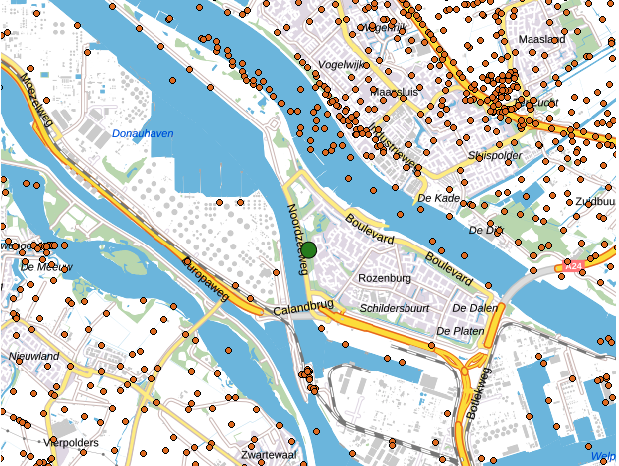
\includegraphics[width=0.40\linewidth]{figures/roz/boor.png}
    \caption{Profile of geological formations and interpretation of formations of Rozenburg. Coordinates of the site of the drill profile are x, y 75250, 436180 (Ondergrondgegevens | DINOloket, 2023).}
\end{figure}\\
\\
\begin{figure}[htbp]
    \centering
    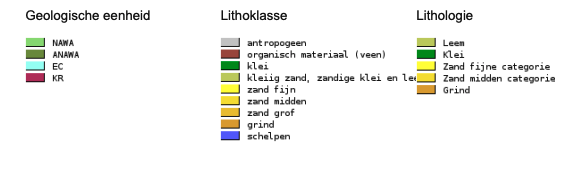
\includegraphics[width=0.40\linewidth]{figures/roz/litho.png}
    \caption{Legend of the geological units and lithological classifications (Ondergrondgegevens | DINOloket, 2023).}
\end{figure}\\
\newpage
The location of the exact drill profile is shown in figure 4.4. As can be seen in the figure, the location is in the southwestern side of the neighborhood, close to the connecting road. \\
\\
\begin{figure}[htbp]
    \centering
    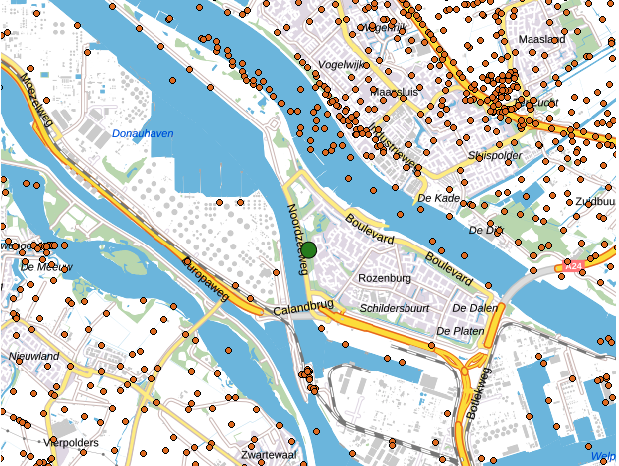
\includegraphics[width=0.40\linewidth]{figures/roz/drillsite.png}
    \caption{Exact location of the drill profile. Coordinates of the site of the drill profile are x, y 75250, 436180 (Ondergrondgegevens | DINOloket, 2023).}
\end{figure}\\
\\
As stated by CBS (2020),  total surface area of Rozenburg counts up to 411 hectares in total, of which 324 hectares are made of land. Since the municipality is only responsible for the public terrain, monitoring wells that are located on private terrains are not considered. 1576 m2 of the 32400 m2 is considered public terrain (CBS, 2020). Rozenburg has 29 phreatic monitoring wells, meaning that there is roughly 1 monitoring well per 54.34 m2 present in the area. In figure 4.5, a geographical representation of the neighborhood Rozenburg is displayed. Points of interest are the blue marked points, which indicate the available phreatic monitoring wells in the neighborhood. \\
\\
\begin{figure}[htbp]
    \centering
    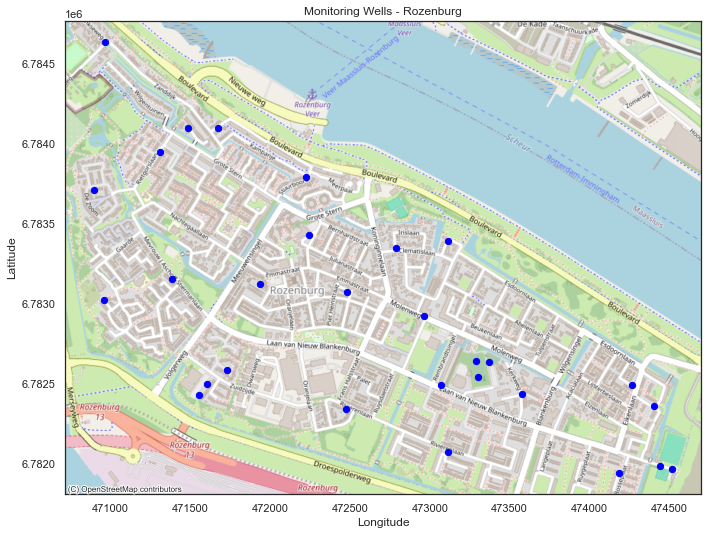
\includegraphics[width=0.75\linewidth]{figures/roz/basic_roz.png}
    \caption{Distribution of monitoring wells or also called the groundwater monitoring network of Rozenburg (Author's own contribution).}
\end{figure}\\
\\
\newpage
\\
\subsection{Heijplaat}
%Tuindorp Heijplaat = garden village Heijplaat
Since the mid-15th century, the hamlet "de Heij" was located at the northern side of the neighborhood "Charlois". At the north of the hamlet, the creek "de Koedood" flew into the Meuse, see figure 4.6. However, years later, an industrial area called "de Heijsehaven" was constructed at that site, where an artificial sand formation was formed as well. Only at the beginning of the 20th century, the idea of the garden village arose (Sebregts, 2019). Throughout the years, the village became more isolated because of the extension of the industrial areas. Heijplaat is still surrounded by industrial areas and water. Access to Heijplaat is solely possible through one entrance road, the Waalhavenweg. At the end of 2023, it emerged that the neighborhood experiences issues with the establishment of a new waste management firm. Additionally, water-related problems have been documented in the historic center as well. Construction initiatives have been proposed to address these issues with a focus on replacing the sewage system as a solution to the water-related inconveniences (Gemeente Rotterdam, 2023). \\
\begin{figure}[h]
    \centering
    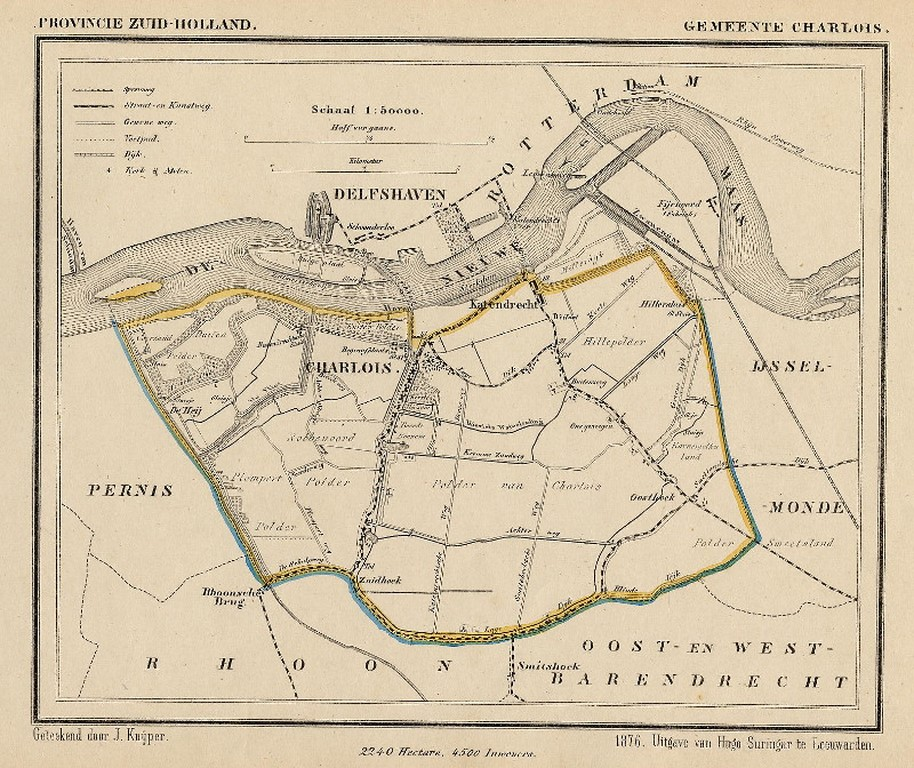
\includegraphics[width=0.40\linewidth]{figures/heij/charloisdeheij.jpeg}
    \caption{Geographical representation of the former hamlets: Charlois, Pernis, and the Heij (Suringar, 1867).}
\end{figure}\\
\\
\newpage

Figure 4.7 and 4.8 describe the lithology of Heijplaat. The subsurface in the eastern part consists of deposits from the formations Dunkirk III, Dunkirk I, and peat. The western part, however, is characterized by the formation of Dunkirk III only on top of a peat layer. In the period between the 10th and 12th century A.P., the peat area has been drained and resulted in a drop of the ground level, making the construction of dikes necessary. The Riederwaard dike, originally located in the neighborhood IJsselmonde, might appear in the area of Heijplaat. Several storm surges ensured that the Riederwaard dike was destroyed. Measures to re-dike the Riederwaard overlaps centuries. Therefore, sections of the dike are identified more downstream. Heijplaat is an example for this (Gemeente Rotterdam, 2013). 

\begin{figure}[htbp]
    \centering
    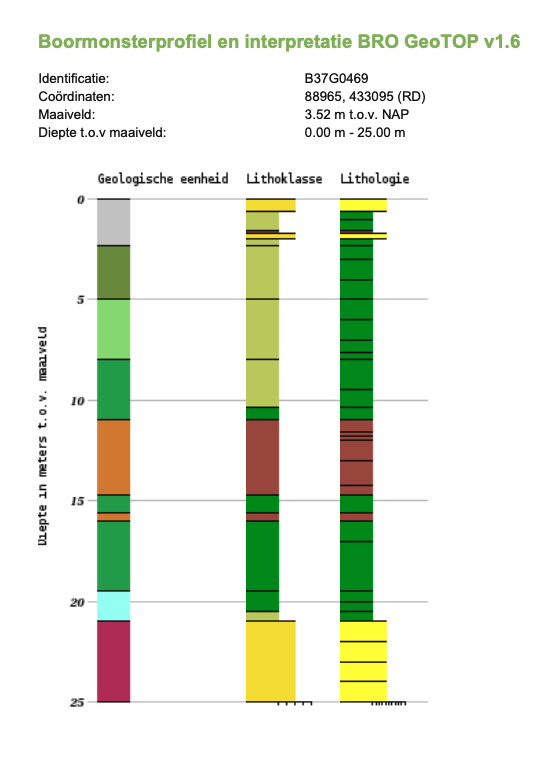
\includegraphics[width=0.40\linewidth]{figures/heij/drillsite.png}
    \caption{Profile of geological formations and interpretation of formations of Heijplaat. Coordinates of the site of the drill profile are x, y: 88529, 433870 (DINOloket, 2023).}
\end{figure}
\begin{figure}[htbp]
    \centering
    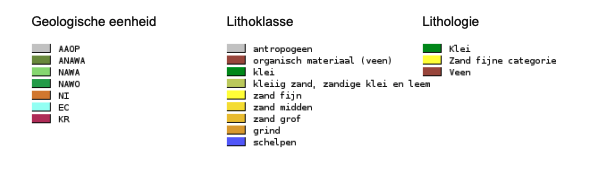
\includegraphics[width=0.40\linewidth]{figures/heij/litho.png}
    \caption{Legend of the geological units and lithological classifications (DINOloket, 2023).}
\end{figure}


\begin{figure}[htbp]
    \centering
    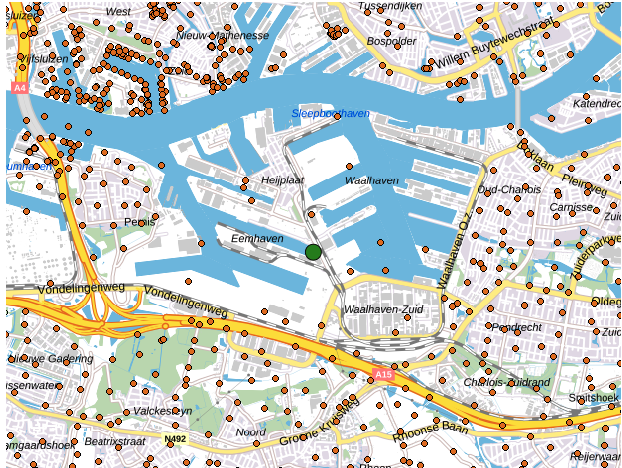
\includegraphics[width=0.40\linewidth]{figures/heij/boor.png}
    \caption{Exact location of the drill profile. Coordinates of the site of the drill profile are x, y: 88529, 433870 (DINOloket, 2023).}
\end{figure}

The total surface area of Heijplaat counts up to 39 hectares in total, of which 39 hectares are also made of land (CBS, 2020). Only 157 m2 of the surface area is public terrain, meaning that there is 1 monitoring well present per 11.21 m2 according to CBS (2020). Figure 4.10, visualizes a geographical representation of the neighborhood Heijplaat, part of Charlois. Points of interest are the blue marked points. They indicate the available phreatic monitoring wells in Heijplaat. 
\begin{figure}[htbp]
    \centering
    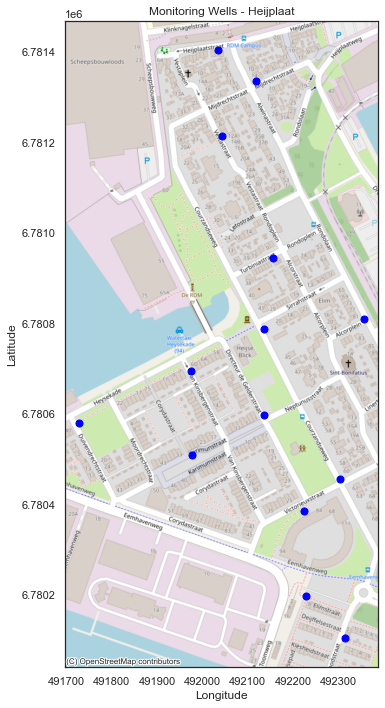
\includegraphics[width=0.40\linewidth]{figures/heij/basicheij.png}
    \caption{Distribution of monitoring wells or also called the groundwater monitoring network of Heijplaat (Author's own contribution).}
\end{figure}


%Beide 3e verdieping Rdam collectie: 
%Heijplaat: HEIJ
%Rozenburg: ROOV 


%Buitendijks of binnendijks gebied? 
%Volgens watertoets ligt het plangebied van Heijplaat grotendeels buitendijks.